\newpage
\section{Animations}
Two important concepts in animations are \textbf{Quaternions} and \textbf{Bezier Curves}

\subsection{Quaternions}
When dealing with movements considering Euler angle rotations the \textbf{gimbal lock} represented an important problem : it causes to loose one degree of freedom due to the alignment of two rotating axis in the same direction. This phenomenon causes \textbf{unrealistic movements}. \textbf{Quaternions} are a solution to this problem : it encodes a rotation in space with \textbf{4 numbers} linearly dependent ( instead of 3).\\
Quaternions are \textbf{extensions} of complex numbers that have \textbf{three imaginary components}:
\begin{itemize}
\item Complex number $\rightarrow$ $a+ib$
\item Quaternions $\rightarrow$ $a+ib+jc+kd$ where the three imaginary components are called \textbf{vector part} subject to the following relation $$ i^2 + j^2 + k^2 = ijk = -1$$ $$ i \cdot j = k  $$ $$... $$
\end{itemize}
A complete algebra can be defined with Quaternions : 
\begin{itemize}
\item Sum of two quaternions $$ (a_1+ib_1+jc_1+kd_1)+(a_2+ib_2+jc_2+kd_2) = (a_1+a_2)+i(b_1+b_2)+j(c_1+c_2)+k(d_1+d_2)$$
\item Product with scalar $$ \alpha(a+ib+jc+kd)= \alpha a+i\cdot \alpha
 b + j\cdot \alpha c + k\cdot \alpha d$$
\item Product of two quaternions
 \begin{align*}
(a_1+ib_1+jc_1+kd_1)(a_2+ib_2+jc_2+kd_2) = (a_1a_2-b_1b_2-c_1c_2-d_1d_2)\\+i(a_1b_2+b_1a_2+c_1d_2-d_1c_2)\\+j(a_1c_2+c_1a_2+d_1b_2-b_1d_2)\\+k(a_1d_2+d_1a_2+b_1c_2-c_1b_2)
\end{align*}
\item Norm $$ ||a+ib+jc+kd||= \sqrt{a^2+b^2+c^2+d^2}$$
\item Angle $$ \theta = arcos\frac{a}{\sqrt{a^2+b^2+c^2+d^2}} $$
\item Rising to power $\alpha$ $$ (a+ib+jc+kd)^{\alpha}= ||a+ib+jc+kd||^{\alpha}\left( cos(\alpha \theta)+ \frac{ib+jc+kd}{\sqrt{b^2+c^2+d^2}}sin(\alpha \theta)\right)$$
\item Unitary quaternions $$ ||a+ib+jc+kd||= \sqrt{a^2+b^2+c^2+d^2} = 1$$
\end{itemize}
Quaternions can encode rotations in 3D of an angle $\theta$ along an axis oriented along a \textbf{unitary} vector $v=(x,y,z)$ : 
\[
\boxed{q= cos \frac{\theta}{2} + sin \frac{\theta}{2} (ix+jy+kz)}
\]
Since v is unitary also \textbf{q is unitary}.
For example a rotation along the x-axis only ( v= (1,0,0)):
$$ q= cos \frac{\theta}{2} + isin \frac{\theta}{2} $$
If two unitary quaternions $q_1 q_2$ encode two different rotations  then their product encodes the composed form : $$ M_1 \Leftrightarrow q_1 \quad M_2 \Leftrightarrow q_2 \to M_1 \cdot M_2 \Leftrightarrow q_1 \cdot q_2$$
This way Euler angles can be transformed into a quaternion:
$$ R = R_y(\Phi) \cdot R_x(\theta) \cdot R_z(\phi)$$
\[
\boxed{q=\left( cos \frac{\psi}{2}+jsin \frac{\phi}{2}\right) \left( cos \frac{\theta}{2}+isin \frac{\theta}{2}\right)\left( cos \frac{\phi}{2}+ksin \frac{\phi}{2}\right)}
\]
where
\begin{align*}
q= \left( cos \frac{\psi}{2} cos \frac{\theta}{2} cos \frac{\phi}{2}- sin \frac{\psi}{2}sin \frac{\theta}{2} sin \frac{\phi}{2} \right) \\
+i\left( cos \frac{\psi}{2} sin \frac{\theta}{2} cos \frac{\phi}{2}- sin \frac{\psi}{2}cos \frac{\theta}{2}sin\frac{\phi}{2}\right) \\
+j \left( sin \frac{\psi}{2} cos \frac{\theta}{2} cos \frac{\phi}{2}- cos \frac{\psi}{2}sin \frac{\theta}{2}sin\frac{\phi}{2}\right)\\
+k \left( cos \frac{\psi}{2} sin \frac{\theta}{2} cos \frac{\phi}{2}- sin \frac{\psi}{2}sin \frac{\theta}{2}cos\frac{\phi}{2}\right)
\end{align*}
The opposite operation where $q=a+ib+jc+kd$ can be easily converted into a \textbf{rotation matrix} :

$$ R= \begin{bmatrix}
    1-2c^2-2d^2       & 2bc+2ad & 2bd-2ac  & 0 \\
    2bc-2ad      & 1-2b^2-2d^2 & 2cd+ 2ab & 0 \\
    2bd+2ac       & 2cd-2ab & 1-2b^2-2c^2 & 0 \\
    0 & 0 & 0 & 1 
\end{bmatrix}$$

\subsection{Bezier Curves}
Bezier curves are \textbf{non-linear interpolation technique} that uses several intermediate points to control the shape of the curve.Their are characterized by their degree : \textbf{linear} ,\textbf{quadratic} , \textbf{cubic}...\\
Bezier curves of degree N are defined by \textbf{N+1 values} and are computed in a \textbf{recursive} way. Consider a  linear interpolation ( function similar to the one see in the first chapters ) between two values a and b at intermediate point $\alpha \in [0,1]$ $$ lerp(a,b,\alpha )=  (1-\alpha)a+\alpha b = I(0,\alpha,1,a,b )$$
A Bezier curved of degree N defined by points $x_0,...,x_N$ passes in $x_0 \text{ at } \alpha =0 $ and in $x_N \text{ at } \alpha =1$ . The function $Bezier_n(x_0,...,x_N,\alpha)$ returns the value of the Bezier curve of degree n at intermediate point $\alpha$ :
\[
\boxed{Bezier_1(x_0,x_1,\alpha)=lerp(x_0,x_1,\alpha)}
\]
\[
\boxed{Bezier_N(x_0,...,x_N,\alpha)= lerp(Bezier_{N-1}(x_0,...,x_{N-1},\alpha),Bezier_{N-1}(x_1,...,x_{N},\alpha),\alpha) }
\]
So for N points the Bezier functions split the set in two :
\begin{itemize}
\item from $x_0 \to x_{N-1}$
\item from $x_1 \to x_{N}$ 
\end{itemize}
And the applied the \texttt{lerp} function with those two as first two arguments.
For example in a cubic curve : 
$$ x_{01} = lerp(x_0,x_1,\alpha)$$
$$ x_{12} = lerp(x_1,x_2,\alpha)$$
$$ x_{23} = lerp(x_2,x_3,\alpha)$$
$$ x_{012} = lerp(x_{01},x_{12},\alpha)$$
$$ x_{123} = lerp(x_{12},x_{23},\alpha)$$
$$ Bezier(x_0,x_1,x_2,x_3,\alpha) = lerp(x_{012},x_{123},\alpha)$$
 \begin{figure}[H]
 \centering
 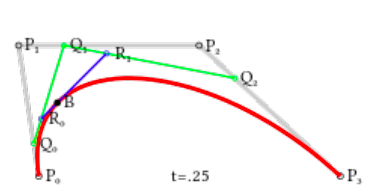
\includegraphics[width=.5\linewidth]{bezier} 
 \end{figure}